%\documentclass[12pt,a4paper]{article}
\documentclass[letterpaper,12pt,titlepage]{article}

\usepackage{hyperref}
\usepackage{listings}
\usepackage{wasysym}
\usepackage{graphicx}


\hypersetup{
	colorlinks,
	citecolor=black,
	filecolor=black,
	linkcolor=black,
	urlcolor=black
}

% This is a comment
\title{Software Requirements and Planning}
\author{
  \texttt{Sarahi Pelayo (pelayos)}
  \\[.5ex]
  \texttt{Katherine Jeffrey (jeffreyk)}
  \\[.5ex]
  \texttt{Megan Bigelow (bigelowm)}
  \\[.5ex]
  \texttt{Johnathan Lee (leejohna)}
  \\[.5ex]
  \texttt{Jonathan Rohr (rohrj)}
}

\begin{document}
\maketitle

\section{Project Description}
Many people experience mental and physical trauma from Sexual Assault, PTSD, Abuse, and Depression, but they might not know how to handle it. If they don’t have people in their lives they can talk to or access to professional help they might not know what to do. It’s important for victims to understand what’s happened to them so they can find ways to effectively deal with it. To solve these problems we can create a mobile app that shows users facts about these mental disorders and gives them options for connecting with professional help.
\newline
\newline
To combat intrusion we are implementing a passcode to unlock the application which sets us apart from previous approaches. The first page will have a spot for the user to enter their pin number to open the app. The pin can be set in the phone’s app settings. The user gains awareness about their mental health state through the resources without having to type it into their more frequented search engines. The application avoids the user having to erase the history of websites they visit by keeping it private. Users can have the application on their phone without fearing other people could see it and assume they are dealing with depression, PTSD, or trauma from sexual abuse helping alleviate potential stigma. Users who may be experiencing domestic abuse can have the security that access to the application won't be granted even if an abuser is monitoring their phone activity.
\newline
\newline
The home page will tell users to contact 911 in an emergency and also give the numbers of a suicide hotline and poison control. Having these on the first page will quickly get this information to people in immediate danger. The application will provide shortcuts to three main features. 
\newline
\newline
First, access to information which will have pages on abuse, sexual assault, PTSD, and depression with lists of common symptoms, potential causes, health risks, and remedies. The second feature will be resources including contact information for helpline  numbers, support groups, and what to say to operators. There will also be information for resources such as shelters for abuse victims, advice for friends and family of victims, and anonymous support groups. Third is the symptoms log that will let users select how they’re feeling from lists of symptoms on specific dates. This will help users process what they’re feeling and track how their symptoms change over a period of time.
\newline
\newline
The application’s goal of helping the user happens through gaining awareness by learning about PTSD, sexual assault, depression, and how that affects them, then taking action whether it be gaining professional help or selfcare all while being as private and stigma free as possible.
\newline
\newline
\textbf{What programming languages or tools will we use?}
\begin{itemize}
  \item Android Studio
  \item Java language
  \item Github
\end{itemize}
We chose to use Android studio because a team member had positive previous experience. Java was chosen because there is a lot of online resources and documentation on how to use it to develop mobile application. Github will be used for version control and easy of combining code development from multiple team members.
\newline
\newline
\textbf{Functional requirements}
\begin{itemize}
  \item Set up a passcode 
  \item Asking for passcode
  \item Re-prompting for the passcode if it is incorrect
  \item Emergency numbers on the front page will call
  \item The app asked the user if they are sure they want to dial the number
  \item Shortcut to information scroll menu with categories
  \item Shortcut to resources scroll menu with categories
  \item Shortcut to symptom log
\end{itemize}
\noindent
\textbf{Non-functional requirements}
\begin{itemize}
  \item Should be able to initiate an outgoing call
  \item Responsive (3sec or less to unlock)
  \item Doesn’t crash
  \item Menus aren’t cluttered
\end{itemize}
Other documentation provided to users to help understand our system will be upon the initial download. A how to guide will prompt the user to create their passcode and point out some main features.
\newline
\newline
\textbf{Major Features}
\begin{itemize}
  \item App locked by passcode
  \item Emergency information page with shortcut
  \item Resources page with shortcut
  \item Symptom Log with shortcut
\end{itemize}
\textbf{Optional Features}
\newline
\newline
As an optional feature we hope to implement a tailored information page based on their symptom logs. Another optional feature would be an additional category in the resources menu that is called self-help. This option will have links to stress coping mechanisms, links to mediation,  and self care tips.
\newpage

\section{Use Cases}
\textbf{Use Case Name:} PTSD: Natural Disaster
\newline
\newline
\textbf{Goal:} Allows the user to log their symptoms
\newline
\newline
\textbf{Actor:} User with PTSD
\newline
\newline
\textbf{Preconditions:}
\begin{itemize}
\item User has lost someone in the natural disaster
\item User is experiencing symptoms of PTSD like flashbacks
\item User has a cell phone
\item User has the WellLiv application downloaded
\end{itemize}
\textbf{Postconditions:}
\begin{itemize}
\item User has logged their symptoms to the system log
\end{itemize}
\textbf{Flow of Events:}
\begin{itemize}
\item User opens the WellLiv application and is asked to enter a passcode
\item User enters their passcode using the on screen numpad
\item The app attempts to verify the passcode
\item If the passcode is correct, the main page opens
\item If the passcode is incorrect, the app asks the user for the passcode again
\item On the main page, the user clicks the Symptoms log modal and the app brings them to another page
\item User can view previous entries or log new one. User chooses to log new symptoms.
\item User writes about what symptoms they are experiencing or how they are feeling and the app saves it to the database.
\item When the user is finished, they close the app
\item Before shutting off, the app reactivates the locking mechanism
\end{itemize}
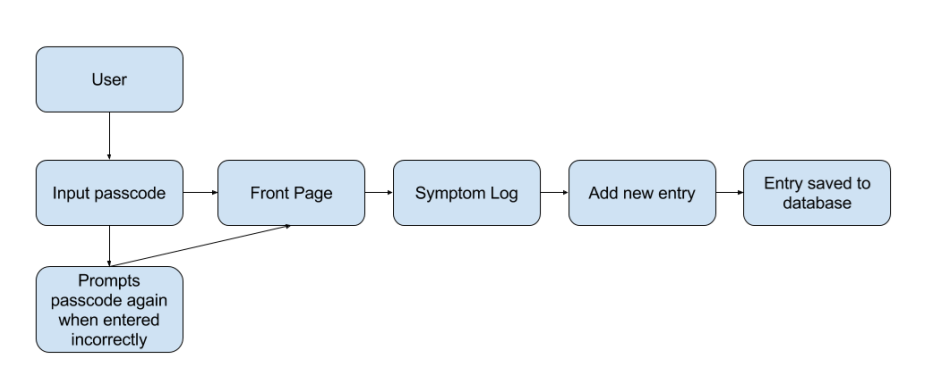
\includegraphics[scale=.4]{Case1}
\newline
\newline
\textbf{Use Case Name:} Sexual Assault
\newline
\newline
\textbf{Goal:} Allow the user quick access to resources such as a sexual assault hotline and basic medical information
\newline
\newline
\textbf{Actor:} Person who’s been sexually assaulted or knows someone who’s been sexually assaulted
\newline
\newline
\textbf{Preconditions:}
\begin{itemize}
\item User has lost someone in the natural disaster
\item User is experiencing symptoms of PTSD like flashbacks
\item User has a cell phone
\item User has the WellLiv application downloaded
\item Someone’s been sexually assaulted
\end{itemize}
\textbf{Postconditions:}
\begin{itemize}
\item User has called appropriate resources to help whoever’s in need
\end{itemize}
\textbf{Flow of Events:}
\begin{itemize}
\item User opens the WellLiv application and is asked to enter a passcode
\item User enters their passcode using the on screen numpad
\item The app attempts to verify the passcode
\item If the passcode is correct, the main page opens
\item If the passcode is incorrect, the app asks the user for the passcode again
\item On the main page, the user clicks the Resources modal and the app brings them to another menu
\item User selects the sexual assault option and the app brings the user to the page with information about various hotlines to call
\item User can access basic medical information, facts, and links to websites which the app stores in a database
\item When the user is finished, they close the app
\item Before shutting off, the app reactivates the locking mechanism
\end{itemize}
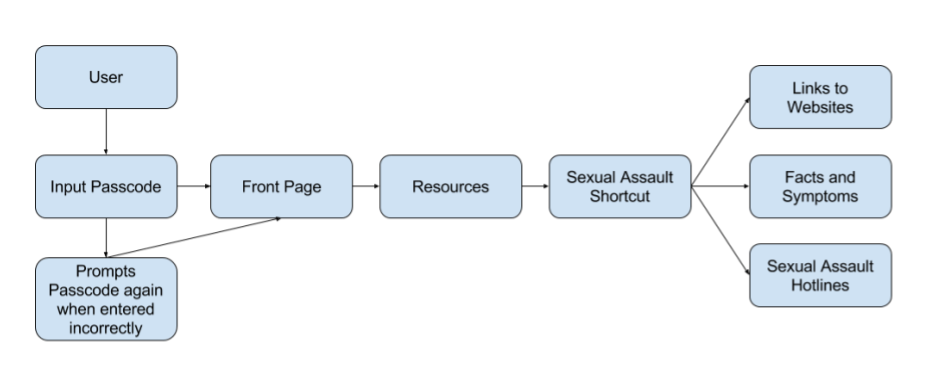
\includegraphics[scale=.4]{Case2}
\newpage
\noindent
\textbf{Use Case Name:} Helping a Suicidal Friend
\newline
\newline
\textbf{Goal:} Allow the user quick access to emergency resources such as poison control center and a suicide hotline, or 911. Also displays basic information needed for self-diagnosis of various situations.
\newline
\newline
\textbf{Actor:} Witness to an incapacitated person or someone who’s suicidal
\newline
\newline
\textbf{Preconditions:}
\begin{itemize}
\item User has a cell phone
\item User has the WellLiv application downloaded
\item Someone is suicidal
\end{itemize}
\textbf{Postconditions:}
\begin{itemize}
\item User is well informed of the situation
\item User has called appropriate resources to help them in their time of need
\end{itemize}
\textbf{Flow of Events:}
\begin{itemize}
\item User opens the WellLiv application and is asked to enter a passcode
\item User enters their passcode using the on screen numpad
\item The app attempts to verify the passcode
\item If the passcode is correct, the main page opens
\item If the passcode is incorrect, the app asks the user for the passcode again
\item On the main page, the user locates the Emergency Phone Numbers section
\item User selects which number they want to call and the app calls the  number (The use can also call it manually).
\item When the user is finished, they close the app
\item Before shutting off, the app reactivates the locking mechanism
\end{itemize}
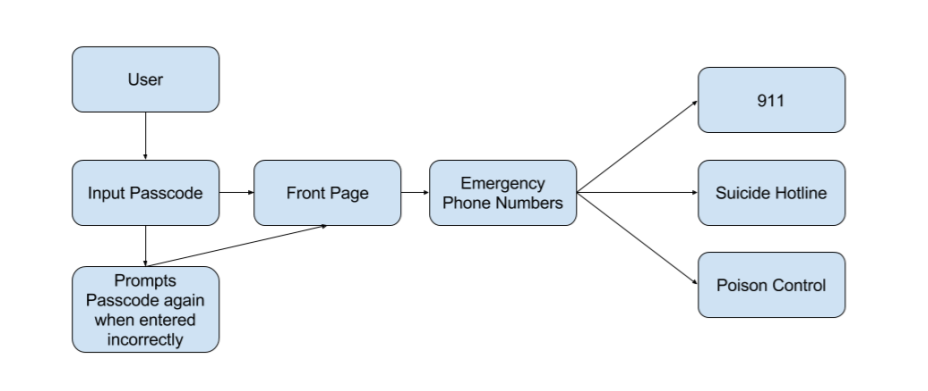
\includegraphics[scale=.4]{Case3}
\newline
\newline
\textbf{Brief Arguments}
\newline
\newline
There are lots of different scenarios that are equally as important as the three covered, but in terms of getting help immediately, the three cases above provide great examples of how the user can access appropriate resources in a short amount of time. 
\newline
\newline
The first use case covers scenarios where a user is aware that they are exhibiting symptoms of PTSD, for example, depression or sexual assault and wants to track their symptoms through the use of the symptom log feature.
\newline
\newline
The following use case covers someone wanting to learn more about what they are experiencing  because they may not be sure what they experienced constitutes as sexual assault, PTSD or depression. Using the information feature of the application they explore definitions and information on their topic of interest while reflecting on their experience. After this gained awareness the user may choose to get professional or selfcare help form the resources shortcut.  
\newpage
\noindent
In the last use case, it covers the scenario where the user needs quick access to emergency phone numbers to help themselves or another person. Access to emergency hotlines covers scenarios, such as, someone who is suicidal can access the suicide hotline and someone who has attempted suicide or knows someone who has attempted suicide via a substance may access the poison control hotline or 911. This case covers scenarios where the user themselves needs access to an emergency number or if someone else is in need.
\newline
\newline
\textbf{Main Error Scenarios}
\newline
\newline
One main error scenario is if the user fails to enter the correct passcode. The app will identify that the entered passcode is incorrect and re-prompt the user until they enter the correct passcode. Another main error scenario is where the user is offline. If that’s the case, a remedy for that is having the app download the necessary information beforehand so that the resources are stored offline. Lastly, if there is a faulty emergency phone number, that will be addressed by first testing that the provided phone numbers for resources work as they are intended and updating them as needed. 
\newpage

\section{Planning}
\textbf{Milestones and tasks:}
\newline
\newline
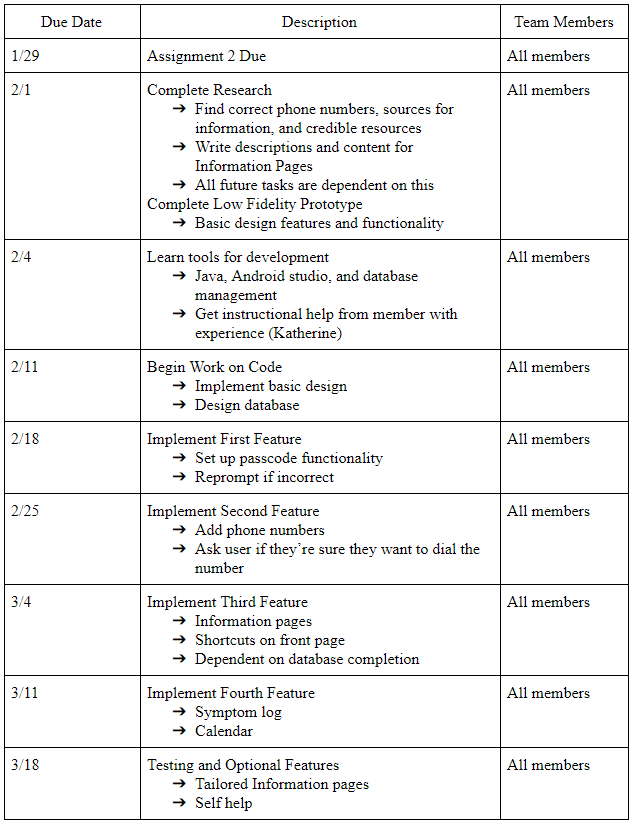
\includegraphics[scale=.796]{Table1}
\newpage
\noindent
\textbf{Project Tracking}
\newline
\newline
We will use the Git and Github to track each members contributions to the coding portion of the project as well as the google doc feature that shows how much each member has contributed to reports.
\newline
\newline
\textbf{Risk Management}
\newline
\newline
The following risks to the project could lead to delays in the delivery of the app.
\newline
\newline
\underline{Risk 1:} Very little experience in Java and database management.
\newline
\underline{Solution:} Spend time learning about Java and database management from a team member who is knowledgeable about it. We could then practice coding in Android Studio to further reduce this risk and become more adept at coding in Java and using the Android Studio interface.
\newline
\newline
\underline{Risk 2:} Other classes, projects and jobs (having a busy schedule) could occupy group members’ time. Also, the time to complete the project could be too short.
\newline
\underline{Solution:} To reduce this risk we could ensure that the workload is split as necessary and to stick to the timeline. In addition to this at least two team members will be knowledgeable in any special skill needed for completing the project.
\newline
\newline
\underline{Risk 3:} Lack of credible information and resources are not up to date.
\newline
\underline{Solution:} To reduce this risk we could dedicate time to researching definitions, statistics, symptoms, and other information that must be correct and unbiased. During this research phase, facts will be double checked through a minimum of  two credible sources before being used in the application.
\newpage
\section{Meeting Report}
\textbf{This Week}
\newline
\newline
\underline{First meeting:} 1/25 in person after class, 5:30pm-5:45pm
\begin{itemize}
\item Members present: Sarahi Pelayo, Katherine Jeffrey, Jonathan Rohr, Johnathan Lee
\item Discussed: We introduced ourselves and exchanged contact information in case of emergency. We then talked about assignment 2.
\item Progress: Google hangouts group chat was set up. Google docs for assignment was set up. Basic elements of the assignment were outlined.
\item Plans: Work on assignment 2.
\item Customers were willing and able to meet 
\end{itemize}
\noindent
\underline{Second meeting:} 1/28 in Google Hangouts, 12pm-3pm
\begin{itemize}
\item Members Present: Sarahi Pelayo, Katherine Jeffrey, Jonathan Rohr, Johnathan Lee
\item Discussed: We discussed assignment 2 with emphasis on use case diagrams, planning timeline, functional features and decided on tools for app development. We decided the project would be worked on in Android Studio using Java. We outlined some of the features we wanted to implement and planned times when we were going to design the prototype.
\item Progress: The project description was fully typed out and three use cases were constructed. Diagrams for the use cases were then drawn up to help demonstrate the process. A timeline for the project was organized with dates and goals. Risks to the project were assessed and planned for. 
\item Plans: Finish assignment 2, start research, and prototype development.
\item Customers were willing and able to meet
\end{itemize}
\textbf{Next Week}
\newline
\newline
Plans and goals:
\begin{itemize}
\item Create comprehensive list of all the topic of information needed.
\item Talk about the prototype design. 
\item Assign who will make the prototype.
\item Create a low level prototype of paper with basic features.
\item Divide up the topics and assign to members for research.
\item Research information needed with emphasis on credibility.
\item Create short description for the informational content researched
\end{itemize}

\bibliography{myref}
\bibliographystyle{ieeetr}

\end{document}
